\documentclass{article}
\usepackage[utf8]{inputenc}
\usepackage{graphicx}
\usepackage{listings}

\title{EEL 4712C - Digital Design: Lab Report 0}
\author{Cole Rottenberg \\ 11062528}
\date{\today}

\begin{document}

\maketitle

\section*{Prelab Report}

\subsection*{Prelab Questions}
% Insert prelab questions and answers here

\subsection*{Prelab Design and Implementation}
% Detail the design and implementation of the prelab
\subsubsection*{firstCircuit Implementation:}
\begin{figure}[h]
  \centering
  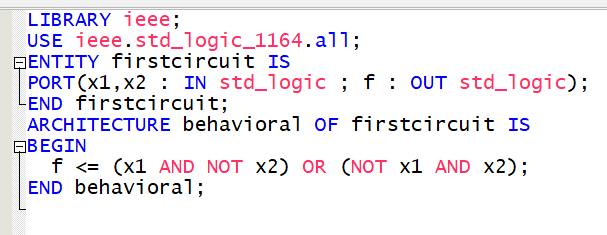
\includegraphics[width=0.75\textwidth]{code.png}
  \caption{firstCircuit Implementation}
\end{figure}

\subsubsection*{Counter Implementation:}
The counter circuit is comprised of 4 components interconnected with a top level entity. The components are: an encoder, a clock divider, a counter, and d flip flops. The encoder takes in the 4 bit counter output and outputs a 7 bit value representing the current count in the 7 segment led. The clock divider takes in the 50MHz clock and outputs a 1Hz clock. The counter takes in the 1Hz clock and outputs a 4 bit value representing the current count. The d flip flops take in the 1Hz clock and the 4 bit counter output and output the 4 bit counter output to the encoder. The top level entity takes in the 50MHz clock and outputs the 4 bit counter output and the 7 bit encoder output. The top level entity also connects the 4 bit counter output to the d flip flops and the 1Hz clock to the counter and d flip flops. \\
\textbf{Encoder:}
\begin{figure}[h]
  \centering
  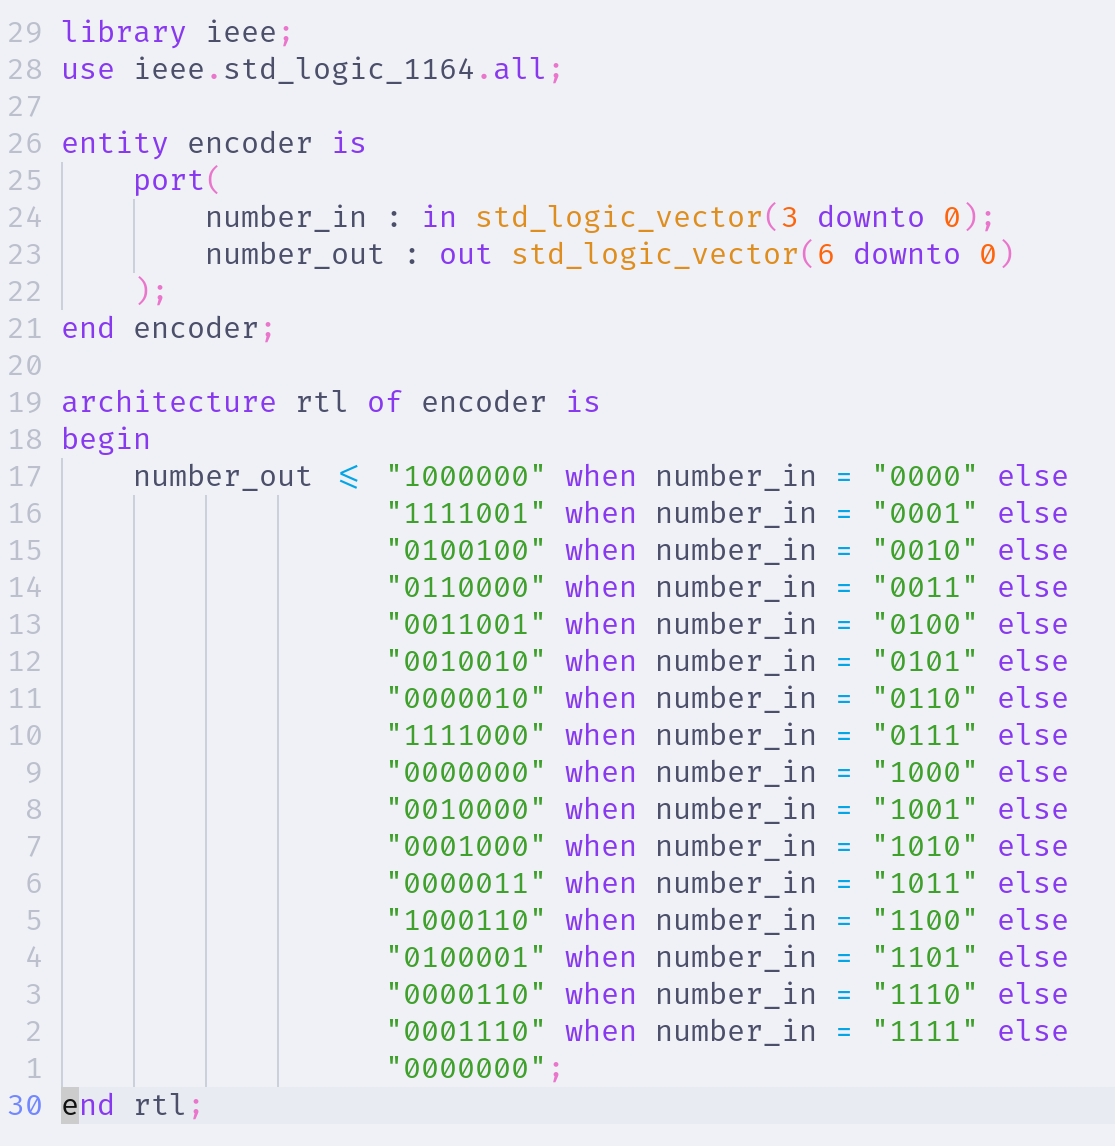
\includegraphics[width=0.75\textwidth]{encoder.png}
  \caption{Encoder Implementation}
\subsection*{Reflection}
% Reflect on the learning and challenges faced during the prelab

\subsection*{Prelab Homework}
% Show all work for the Prelab Homework here
\begin{enumerate}
  \item \textbf{Problem 1:} A\_123, A123\_, c1\_\_c2, and1
  \item \textbf{Problem 2:} All are equivalent.
  \item \textbf{Problem 3:} False.
  \item \textbf{Problem 4:} Sequential logic happens in a sequence of time, while concurrent logic happens at the same time.
  \item \textbf{Problem 5:} 
  \begin{lstlisting}[language=VHDL]
    entity firstCircuit is
      port (a, b, c, d: in std_logic;
            g: out bit);
    end firstCircuit;

    architecture bhv of firstCircuit is
    begin
      e <= a and b;
      f <= c or e;
      g <= d and f;
    end bhv;
  \end{lstlisting}
  \item \textbf{Problem 6:} $X_3$ must be added to the sensitivity list.
  \item \textbf{Problem 7:} \\
  \begin{tabular}{|c|c|c|c|c|c|c|c|}
    \hline
    $X_1$ & $X_2$ & $X_3$ & $C$ & $A$ & $B$ & $D$ & $F$ \\
    \hline
    0 & 0 & 0 & 0 & 1 & 1 & 1 & 0 \\
    \hline
    0 & 0 & 1 & 0 & 1 & 0 & 1 & 0 \\
    \hline
    0 & 1 & 0 & 1 & 0 & 1 & 1 & 1 \\
    \hline
    0 & 1 & 1 & 1 & 0 & 0 & 0 & 0 \\
    \hline
    1 & 0 & 0 & 1 & 1 & 1 & 1 & 1 \\
    \hline
    1 & 0 & 1 & 1 & 1 & 0 & 1 & 1 \\
    \hline 
    1 & 1 & 0 & 1 & 0 & 1 & 1 & 1 \\
    \hline
    1 & 1 & 1 & 1 & 0 & 0 & 0 & 0 \\
    \hline
  \end{tabular}
\end{enumerate}

\section*{Postlab Report}

\subsection*{Problem Statement}
% Provide a short description of the lab’s goals, system, inputs, outputs, and function
% Section should be 1-2 paragraphs

\subsection*{Design}
% Describe the design decisions, components, signals, and algorithms used

\subsection*{Implementation}
% Describe the implementation process, time required, and any relevant code or pictures

\subsection*{Testing}
% Explain how the design was tested and the outcomes

\subsection*{Conclusions}
% Summarize the work, successes, problems encountered, and future improvements

\section*{Appendix}
% Include all postlab code, screenshots, pictures, and simulations here

\end{document}
